\begin{frame}
    \titlepage
\end{frame}

\begin{frame}{questions/logistics}
    \begin{itemize}
    \item office hours posted on website
    \item VM setup due Friday
    \end{itemize}
\end{frame}

\section{Virtual Machine Abstraction}

\begin{frame}{virtual machines}
    \begin{itemize}
    \item illusion of a dedicated machine
    \item could or could not behave like real machine
    \end{itemize}
\end{frame}

\begin{frame}<1>[label=vmTypes]{virtual machine types}
    \begin{itemize}
        \item \myemph<2>{language} --- designed for programming language
        \item \myemph<3>{process} --- designed for shared system
        \item \myemph<4>{system} --- designed to emulate ``real'' hardware 
    \end{itemize}
\end{frame}

\subsection{Language VM}

\againframe<2>{vmTypes}

\begin{frame}{language VMs}
    \begin{itemize}
    \item programming languages have a `virtual machine'
    \item e.g. the Java virtual machine
    \vspace{.5cm}
    \item compiler targets virtual machine
    \item virtual machine \myemph{designed for language}
    \item easier than real machine to compile to
    \item reasonably fast to simulate on real machine
    \end{itemize}
\end{frame}

\begin{frame}{JVM specializations}
    \begin{itemize}
    \item ``assembly'' of virtual machine \\ \myemph{knows about objects, methods}
    \item ISA \myemph{designed for Java programs}
        \begin{itemize}
        \item with some adaptations for other languages
        \end{itemize}
    \item all stack-based instructions (no registers)
        \begin{itemize}
        \item (thought to be) easier to implement in software
        \end{itemize}
    \item \myemph{safe}: can't leak memory; can't segfault
    \end{itemize}
    \begin{tikzpicture}[overlay,remember picture]
        \node[anchor=north east] at (current page.north east) {
            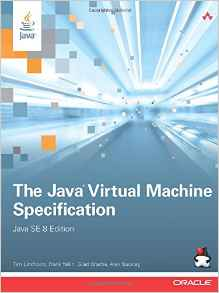
\includegraphics[width=0.2\pagewidth]{jvm-spec-cover}
        };
    \end{tikzpicture}
\end{frame}

\subsection{Process VM}

\againframe<3>{vmTypes}

\begin{frame}{OSs are virtual machines}
    \begin{itemize}
    \item process virtual machines
    \item \myemph{different interface than physical HW}
    \item system calls instead of I/O instructions
    \item system calls/signals instead of interrupts
    \end{itemize}
\end{frame}

\begin{frame}{process versus system}
    \begin{itemize}
    \item more complicated:
        \begin{itemize}
        \item files
        \item network connections
        \item communicating with other processes
        \item \ldots
        \end{itemize}
    \item but simpler to program
        \begin{itemize}
        \item more flexible
        \item no hardware details (disk sizes, etc.)
        \end{itemize}
    \end{itemize}
\end{frame}

\subsection{System VM}

\againframe<4>{vmTypes}

\begin{frame}{system virtual machines}
    \begin{itemize}
    \item acts (more) \myemph{like} real hardware
    \item not files, but a hard drive
    \item not network connections, but an ethernet device
    \item not memory allocation calls, but page tables
    \item \ldots
    \item system virtual machines \myemph{run operating systems}
    \end{itemize}
\end{frame}

\begin{frame}{modern system VM software}
    %FIXME: logos
    \begin{itemize}
    \item VMWare --- 1998 startup
    \item VirtualBox (open source; Oracle, formally Sun)
    \item Parallels (targets OS X)
    \item Xen
    \item QEMU
    \item Hyper-V (Microsoft)
    \end{itemize}
\end{frame}

\begin{frame}{hosts and guests}
    \begin{itemize}
    \item \myemph{guest} OS --- what's inside the virtual machine
    \item \myemph{host} OS --- what's outside the virtual machine
    \end{itemize}
\end{frame}

\begin{frame}{VM implementation strategies}
    \begin{tikzpicture}
    \begin{scope}[yscale=0.78,xscale=1.3]
    \node[anchor=center] at (3, .5) {\bfseries traditional VM};
    \draw[thick] (0, 0) -- (6, 0) -- (6, -1) -- (3, -1) -- (3, -2)  -- (1, -2) -- (1, -3) -- (0, -3) -- cycle;
    \node[anchor=center] at (3, -.5) {virtual machine/guest OS};
    \draw[thick] (6, -3) -- (6, -1) --  (3, -1) -- (3, -2) --  (5, -2) -- (5, -3) -- cycle;
    \node[anchor=center] at (4.5, -1.5) {VM monitor};
    \draw[thick] (1, -2) -- (1, -3) -- (5, -3) -- (5, -2) -- cycle;
    \node[anchor=center] at (3, -2.5) {host OS};
    \draw[thick] (0, -3) -- (0, -4) -- (6, -4) -- (6, -3) -- cycle;
    \node[anchor=center] at (3, -3.5) {native CPU};
    \begin{visibleenv}<2->
        \draw[very thick, orange] (3, -1) -- (6, -1) node[right,orange,align=center] {privileged ops \\ become callbacks \\ (help from HW+OS)};
        %\draw[very thick, red] (5, -2) -- (1, -2) node[left,red,align=center] {system\\ calls};
        \draw[very thick, blue] (0, -3) -- (6, -3) node[right,blue] {native instruction set};
    \end{visibleenv}
        \coordinate (sameNativeLine) at (3, -3);
        \begin{pgfonlayer}{fg}
        \begin{visibleenv}<3>
        \node[mycallout2=sameNativeLine,anchor=north,align=left] at (3, -4) {
            virtual ISA same as real ISA \\
            (except for privileged operations)
        };
        \end{visibleenv}
        \end{pgfonlayer}
    \end{scope}
    \begin{scope}[yshift=-3.9cm,xscale=1.3,yscale=0.78]
    \node[anchor=center] at (3, .5) {\bfseries emulator};
    \draw[thick] (0, 0) -- (6, 0) -- (6, -1) -- (0, -1) -- cycle;
    \node[anchor=center] at (3, -.5) {virtual machine/guest OS};
    \draw[thick] (6, -1) -- (0, -1) -- (0, -2)  -- (5, -2) -- (5, -3) -- (6, -3) -- cycle;
    \node[anchor=center] at (3, -1.5) {emulator};
    \draw[thick] (0, -2) -- (0, -3) -- (5, -3) -- (5, -2) -- cycle;
    \node[anchor=center] at (3, -2.5) {host OS};
    \draw[thick] (0, -3) -- (0, -4) -- (6, -4) -- (6, -3) -- cycle;
    \node[anchor=center] at (3, -3.5) {native CPU};
    \begin{visibleenv}<2->
        \draw[very thick, red] (0, -1) -- (6, -1) node[right,red,align=center] {interpret/translate};
        \draw[very thick, blue] (0, -3) -- (6, -3) node[right,blue] {native instruction set};
    \end{visibleenv}
    \begin{visibleenv}<4>
        \coordinate (diffNativeLine) at (3, -1);
        \node[mycallout2=diffNativeLine,anchor=south,align=left] at (4, 0) {
            virtual ISA could be different from real ISA \\
            (even excluding privileged operations)
        };
    \end{visibleenv}
    \end{scope}
    \end{tikzpicture}
\end{frame}

\section{VM History}

\begin{frame}{VMs are old}
IBM/370 Model 158 (announced 1972) marketing: \\
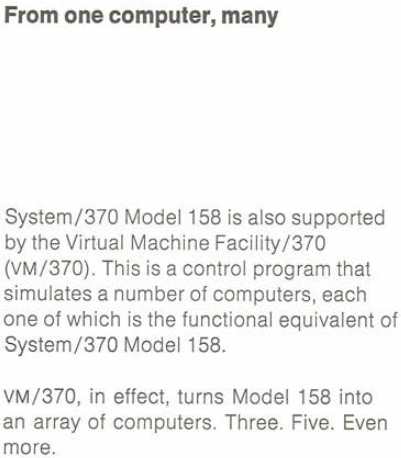
\includegraphics[width=0.4\textwidth]{370-pamphlet-excerpt}\hspace{.5cm}
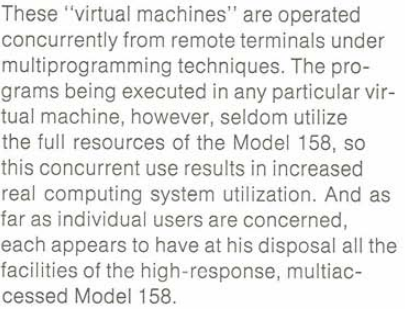
\includegraphics[width=0.4\textwidth]{370-pamphlet-excerpt2}
\imagecredit{Excerpt from: Computer History Museum catalog number 102646258 \\ \url{http://www.computerhistory.org/collections/catalog/102646258}}
\end{frame}

\subsection{IBM VM/370}

\begin{frame}{VMs as consolidation}
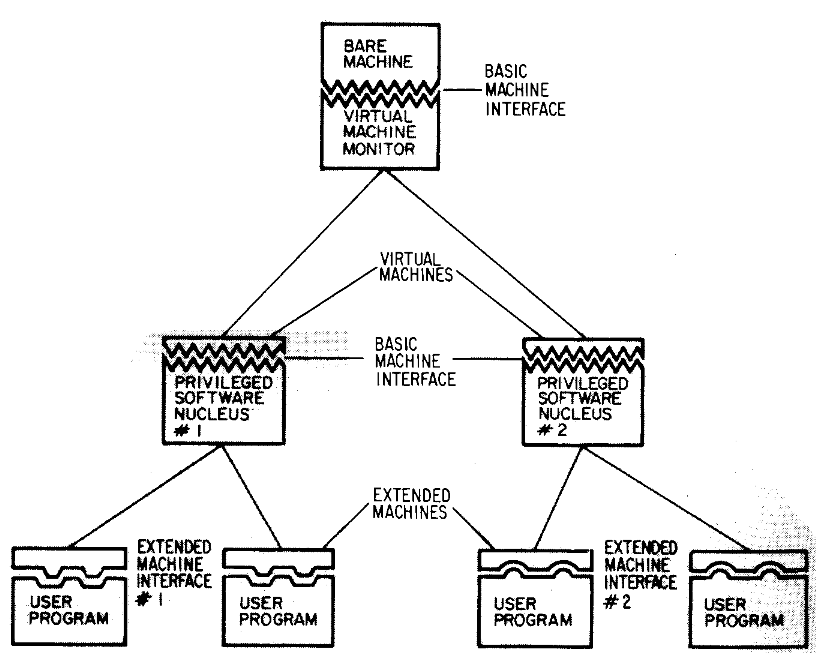
\includegraphics[height=0.8\textheight]{VMSurvey-Fig2}
\imagecredit{Figure: Goldberg, ``Survey of Virtual Machine Research'', IEEE Computer, September 1974}
\end{frame}

\begin{frame}{the consolidation case}
\begin{itemize}
    \item compatibility --- \myemph{customize ``whole'' machine}
    \item efficiency --- 
        \begin{itemize}
        \item two+ CPUs/hard drives for the work/data of one?
        \item two+ CPUs for the work/data of one?
        \end{itemize}
    \vspace{.5cm}
    \item 2011 public `cloud' server CPU utilization: <10\%
        \begin{itemize}
        \item \myemph{after} consolidation
        \end{itemize}
    \imagecredit{utilization \%s: Liu, ``A Measurement Study of Server Utilization in Public Clouds''}
\end{itemize}
\end{frame}

\subsection{Resurgence: VMWare}

\begin{frame}{VM death and resurgence}
\begin{itemize}
\item VMs started with \myemph{mainframes}
\item one computer for \myemph{an entire company}
\item \ldots{}
\item then the personal computer happened
\end{itemize}
\end{frame}

\begin{frame}{resurgence of VMs}
\begin{itemize}
    \item consolidation again (still a good idea)
    \item compatibility 
        \begin{itemize} 
        \item Windows on Mac
        \item Unix on Windows
        \item Windows 98 on Windows NT, etc.
        \end{itemize}
    \item \ldots
    \item 1998 startup: VMWare 
        \begin{itemize} 
        \item bought by EMC which was bought by Dell
        \end{itemize}
\end{itemize}
\end{frame}

\section{VM implementation}

\begin{frame}{VM implementation}
    \begin{itemize}
    \item hardware support --- 
        \begin{itemize}
        \item originally, only viable way
        \item IBM/370, VirtualBox, modern VMware, etc.
        \end{itemize}
    \item binary translation --- 
        \begin{itemize}
        \item historic VMware
        \end{itemize}
    \item paravirtualization --- Xen
    \item emulation --- Bochs
    \end{itemize}
\end{frame}

\begin{frame}{on kernel mode}
    \begin{itemize}
    \item hardware has two modes:
        \begin{itemize}
        \item \myemph{user mode} and \myemph{kernel mode}
        \end{itemize}
    \item typically, only OS can run in kernel mode
    \item \myemph{privileged operations require kernel mode}
    \end{itemize}
\end{frame}

\begin{frame}{exceptions and VMs}
    \begin{itemize}
    \item privileged operations need to run in \myemph{kernel mode}
    \item guest OS is run in \myemph{user mode}
    \item guest OS tries to do a privileged operation? 
        \begin{itemize}
        \item \textit{exception} gives control to host OS
        \end{itemize}
    \item I/O device (e.g. keyboard) tries to signal OS
        \begin{itemize}
        \item \textit{exception} gives control to host OS
        \end{itemize}
    \item exception handlers are part of virtual machine monitor
    \end{itemize}
\end{frame}

\begin{frame}{VMs and kernel mode}
    \begin{itemize}
    \item basic idea: run guest OS in user mode
    \item virtual machine monitor (VMM) runs in kernel mode
    \item on exception: virtual machine monitor \myemph{forwards} to guest OS
    \item ``mirrors'' what hardware did for VMM
    \end{itemize}
\end{frame}

\begin{frame}{system call flow}
\begin{tikzpicture}
\tikzset{
    userProg/.style={fill=green!20!white},
    innerOS/.style={fill=blue!20!white},
    outerOS/.style={fill=yellow!20!white},
}
\matrix[tight matrix,nodes={align=center,text width=9cm,minimum height=1.7cm,execute at begin node=\strut},
    label={[inner sep=1mm]north:conceptual layering}] (layering) {
    |[userProg]| {program \\ ~} \\
    |[innerOS]| {`guest' OS \\ ~} \\
    |[outerOS]| {virtual machine monitor \\ ~} \\
    hardware \\
};
\begin{visibleenv}<3>
    \node[draw,line width=1mm,blue,fit=(layering-1-1) (layering-2-1),inner sep=-.25mm,
        label={[align=left,blue!80!black]right:user\\mode}] {}; 
    \node[draw,line width=1mm,red,fit=(layering-3-1),inner sep=-.25mm,
        label={[align=left,red!80!black]right:kernel\\mode}] {}; 
\end{visibleenv}
\begin{visibleenv}<2,6>
    \node[draw,line width=1mm,cyan,fit=(layering-1-1),inner sep=-.25mm,
        label={[align=left,cyan!80!black]right:pretend\\user\\mode}] {}; 
    \node[draw,line width=1mm,magenta,fit=(layering-2-1),inner sep=-.25mm,
        label={[align=left,magenta!80!black]right:pretend\\kernel\\mode}] {}; 
\end{visibleenv}
\begin{visibleenv}<4->
\begin{scope}
    \tikzset{
        >=Latex,
        l/.style={very thick,red!90!black},
        every node/.style={
            inner sep=1mm
        }
    }   
    \draw[l,->] ([xshift=-8cm,yshift=.1cm]layering-1-1.south east) -- ([xshift=-7.5cm,yshift=-.4cm]layering-4-1.north east)
        node[above,at start,align=center,xshift=3mm] {system call\\(exception)};
    \draw[l,->] ([xshift=-7cm,yshift=-.4cm]layering-4-1.north east) -- ([xshift=-6.6cm,yshift=.1cm]layering-3-1.south east)
        node[above,xshift=.5cm] { \textbf<5>{run handler} };
    \draw[l,->] ([xshift=-5cm,yshift=.1cm]layering-3-1.south east) -- ([xshift=-4.5cm,yshift=-.2cm]layering-4-1.north east)
        -- ([xshift=-4cm,yshift=.1cm]layering-3-1.south east)
        node[below,midway,align=left] { \textbf<6>{update memory map} };
    \draw[l,->] ([xshift=-2cm,yshift=.1cm]layering-3-1.south east) -- ([xshift=-1.5cm,yshift=-.2cm]layering-4-1.north east)
        node[at start,above left,xshift=.5cm,align=left] {to user mode}
        -- ([xshift=-.8cm,yshift=.1cm]layering-2-1.south east)
        node[at end,above,xshift=-.5cm] { \textbf<5>{run handler} };
\end{scope}
\end{visibleenv}
\end{tikzpicture}
\end{frame}

\begin{frame}{extra hardware support}
    \begin{itemize}
    \item privileged operations becoming exceptions: minimal
    \item hardware can do more:
    \vspace{.5cm}
    \item nested page table lookup
        \begin{itemize}
        \item makes memory mapping changes much faster/simpler
        \end{itemize}
    \item handling of read-only privileged instructions
        \begin{itemize}
        \item e.g. reading ``interrupt enable'' flag
        \end{itemize}
    \item forwarding of some exceptions
        \begin{itemize}
        \item e.g. flag to make syscalls run guest OS
        \end{itemize}
    \end{itemize}
\end{frame}

\begin{frame}{binary translation}
    \begin{itemize}
    \item compile assembly to new assembly
    \vspace{1cm}
    \item works without instruction set support
    \item early versions of VMWare on x86 (before x86 added virtualisation support)
    \item can be used to run one platform on another
    \end{itemize}
\end{frame}

\begin{frame}[fragile,label=binTransIdea]{binary translation idea}
\lstset{
    language=myasm,
    style=small,
    morekeywords={movq,addss,subss}
}
\begin{tikzpicture}
\tikzset{
    code/.style={inner sep=0mm,align=left},
    hiOn/.style={alt=#1{rounded corners,fill=green,fill opacity=0.3,text opacity=1.0}{}},
    markOn/.style={alt=#1{rounded corners,draw,thick}{}},
}
\node[code,markOn=<2>,hiOn=<3>] (bb1) {
\begin{lstlisting}
0x40FE00: addq %rax, %rbx
movq 14(%r14,4), %rdx
addss %xmm0, (%rdx)
...
0x40FE3A: jne 0x40F404
\end{lstlisting}
};
\node[right=.25cm of bb1,visible on=<2>,align=left] {
    divide machine code \\
    into \textit{basic blocks} \\
    (= ``straight-line'' code) \\
    (= code till \\ 
    jump/call/etc.)
};
\node[code,right=.25cm of bb1,visible on=<3>] (bb1New) {
generated code: \\
\begin{lstlisting}
// addq %rax, %rbx
movq rax_location, %rdi
movq rbx_location, %rsi
call checked_addq
movq %rax, rax_location
...
// jne 0x40F404
... // get CCs 
je do_jne
movq $0x40FE3F, %rdi
jmp translate_and_run
do_jne:
movq $0x40F404, %rdi
jmp translate_and_run
\end{lstlisting}
};
\node[code,markOn=<2>,anchor=north west] (bb2) at (bb1.south west){
\begin{lstlisting}
subss %xmm0, 4(%rdx)
...
je 0x40F543
\end{lstlisting}
};
\node[code,markOn=<2>,anchor=north west] (bb3) at (bb2.south west){
\begin{lstlisting}
ret
\end{lstlisting}
};
\end{tikzpicture}
\end{frame}

\begin{frame}[fragile,label=binTransIdea2]{a binary translation idea}
    \begin{itemize}
    \item convert whole \textit{basic blocks}
        \begin{itemize}
        \item code upto branch/jump/call
        \end{itemize}
    \item end with call to {\tt translate\_and\_run}
        \begin{itemize}
        \item compute new \myemph{simulated PC} address to pass to call
        \end{itemize}
    \end{itemize}
\end{frame}

\begin{frame}[fragile,label=binTransIdea3]{making binary translation fast}
    \lstset{style=small,language=myasm,morekeywords={movq}}
    \begin{itemize}
    \item cache converted code
        \begin{itemize}
        \item {\tt translate\_and\_run} checks cache first
        \end{itemize}
    \item patch calls to {\tt translate\_and\_run} to refer directly to cached code
    \item do something more clever than \lstinline|movq rax_location, ...|
        \begin{itemize}
        \item map (some) registers to registers, not memory
        \end{itemize}
    \item ends up being ``just-in-time'' compiler
    \end{itemize}
\end{frame}


\begin{frame}{binary translation? really?}
    \begin{itemize}
    \item early VMWare: focused on little pieces of OS code that couldn't be emulated
        \begin{itemize}
        \item a few instructions that behaved differently to fix
        \end{itemize}
    \item used by Apple to handle changing CPU designs
        \begin{itemize}
        \item not a system VM --- used the native OS mostly
        \end{itemize}
    \item Rosetta: run Power PC on Intel (2005--2011)
    \item Mac 68k emulator: Run Motorola 680x0 on Power PC (1994--2005)
    \end{itemize}
\end{frame}

\begin{frame}{why binary translation?: POPF}
    \begin{itemize}
    \item x86 has an instruction called POPF
    \item pop flags from stack
    \begin{itemize}
    \item condition codes --- {\tt CF}, {\tt ZF}, {\tt PF}, {\tt SF}, {\tt OF}, etc.
    \item direction flag ({\tt DF}) --- used by string instructions
    \item \textbf<2>{\myemph<2>{I/O privilege level}} ({\tt IOPL})
    \item \textbf<2>{\myemph<2>{interrupt enable flag}} ({\tt IF})
    \item \ldots
    \end{itemize}
    \item<2> some flags are \myemph{privileged!}
    \item<2> popf \myemph{\textbf{silently}} doesn't change them in user mode
    \end{itemize}
\end{frame}

\begin{frame}{more binary translation problems}
    \begin{itemize}
    \item PUSHF also bad --- want to pretend interrupts are disabled, e.g.
    \item several more x86 instructions
    \vspace{.5cm}
    \item processor extensions to change these to be virtualizable
    \item mechanism: flag to make them trigger interrupt to virtual machine monitor
    \end{itemize}
\end{frame}

\begin{frame}{other binary translation utility}
    \begin{itemize}
    \item enables other software analysis on unmodified binaries
    \item example: valgrind, debugging tools:   
        \begin{itemize}
        \item memory errors
        \item synchronization bugs
        \item \ldots
        \end{itemize}
    \end{itemize}
\end{frame}

\begin{frame}{paravirtualization}
    \begin{itemize}
    \item only a few pieces of the OS use things like {\tt POPF}
    \item instead: modify OS
    \item called \myemph{paravirtualization}
    \item OS makes \myemph{explicit calls} to virtual machine monitor
    \item very small OS patch
    \item more efficient?
    \end{itemize}
\end{frame}

\begin{frame}{other virtualisation support nits}
    \begin{itemize}
    \item hardware support for \myemph{nested page tables}
    \item alternatives work, but are complex/slower
    \item hardware support for limiting I/O devices
        \begin{itemize}
        \item can safely give VMs I/O device access
        \end{itemize}
    \end{itemize}
\end{frame}

\begin{frame}{emulation}
    \begin{itemize}
    \item read instruction, do what it says, repeat
    \vspace{1cm}
    \item slowest technique, but easiest to implement
    \item easiest to provide detailed debugging information for
    \end{itemize}
\end{frame}


\section{VMs and software analysis}

\begin{frame}{Why do we care about VMs?}
    \begin{itemize}
    \item \myemph{isolation}
    \item run dangerous stuff safely!
    \item analyze dangerous stuff without disrupting it!
    \end{itemize}
\end{frame}

\begin{frame}{isolation: network}
    \begin{itemize}
    \item virtual machines have a ``virtual'' network device
    \vspace{1cm}
    \item easy to make disconnected
    \item provide network of other VMs, not connected to internet
    \item setup custom firewall without extra hardware
    \end{itemize}
\end{frame}

\begin{frame}{isolation: disk}
    \begin{itemize}
    \item virtual machines have ``virtual'' hard drives --- just a file!
    \vspace{1cm}
    \item virus infects files? not anything that matters on the machine
    \item easy to identify what to backup
        \begin{itemize}
        \item even if virus modifies ``hidden'' files
        \end{itemize}
    \item \ldots
    \end{itemize}
\end{frame}

% FIXME: screenshot of snapshot feature in virtualbox

\begin{frame}{snapshots}
    
\includegraphics[width=4cm]{snapshot-icon-vbox}
    \begin{itemize}
    \item virtual disks, virtual memory, \ldots
    \vspace{1cm}
    \item make \myemph{copy} of disk/memory/etc.
    \item e.g. see what damage malware does
    \item go back to before damage happens
    \end{itemize}
\end{frame}

\begin{frame}{snapshot efficiency}
    \begin{itemize}
    \item but aren't snapshots slow???
        \begin{itemize}
        \item copy all of disk, memory
        \end{itemize}
    \item can be done faster:
    \end{itemize}
    \begin{tikzpicture}
    \tikzset{
        sectorList/.style={
                tight matrix,
                nodes={text depth=1mm},
                row 1/.style={nodes={font=\small\bfseries\normalfont}},
                column 1/.style={nodes={font=\small\tt,text width=1.6cm}},
                column 2/.style={nodes={font=\small\tt,text width=2.5cm}},
        },
    }
    \matrix[sectorList,label={north:snapshot 1 updates},
        ] (updatesA) {
        sector \# \& data \\
        15 \& FFF434\ldots \\
        456 \& 0045010\ldots \\
        \ldots \& \ldots \\
    };
    \node[left=.5cm of updatesA,align=center] (updatesANote) {read/write\\ from \\ VM};
    \draw[thick,-Latex,dashed] ([xshift=-.7cm]updatesANote.east) -- (updatesA);
    \matrix[sectorList,label={base disk image},
        right=1cm of updatesA,
        ] (baseA) {
        sector \# \& data \\
        0 \& 00235544\ldots \\
        1 \& 44467520\ldots \\
        2 \& 00000000\ldots \\
        \ldots \& \ldots \\
    };
    \draw[line width=1mm,-Latex,dashed] (updatesA) -- (baseA);
    \begin{visibleenv}<2>
    \matrix[sectorList,label={north:snapshot 2 updates},
        below=1cm of updatesA,
        ] (updatesB) {
        sector \# \& data \\
        15 \& FFF434\ldots \\
        456 \& 0045010\ldots \\
        \ldots \& \ldots \\
    };
    \draw[line width=1mm,-Latex,dashed] (updatesB) -- (baseA);
    \end{visibleenv}
    \end{tikzpicture}
\end{frame}


% FIXME: screenshot from bochs-gdb?

\begin{frame}{debugging support}
    \begin{itemize}
    \item \myemph{hardware} has support for debuggers\ldots
    \item but there are ways of interfering/detecting
    \item virtual machines can ``hide'' these changes
        \begin{itemize}
        \item e.g. slow down in debugger? --- virtual clock
        \end{itemize}
    \item (might require slower implementation technique)
    \item also easy to do whole-machine debugging on VMs
        \begin{itemize}
        \item attach GDB to \myemph{entire VM}
        \end{itemize}
    \end{itemize}
\end{frame}

\begin{frame}{VM replay}
    \begin{itemize}
    \item virtual machines can support \myemph{replay}
    \item rerun something \myemph{exactly the same}
    \item good for debugging
    \vspace{.5cm}
    \item not trivial to implement --- why?
    \end{itemize}
\end{frame}

\begin{frame}[fragile,label=replayChallenge]{VM replay challenges}
    \begin{itemize}
    \item timing and I/O
    \item<2-> need to remember exactly when I/O happens
    \item<2-> need to have virtual clock
    \item<2-> how?
        \begin{itemize}
        \item<3-> log all I/O, timer readings
        \item<3-> read log on replay
        \end{itemize}
    \end{itemize}
\begin{visibleenv}<3->
\begin{Verbatim}[fontsize=\small]
at instruction 100043243: keypress 'a'
at instruction 100483782: time = 100333.3456
at instruction 100688445: network packet '024A...'
\end{Verbatim}
\end{visibleenv}
\end{frame}

\section{VM Escape and Detection}

\begin{frame}{virtual machine escape}
\begin{center}
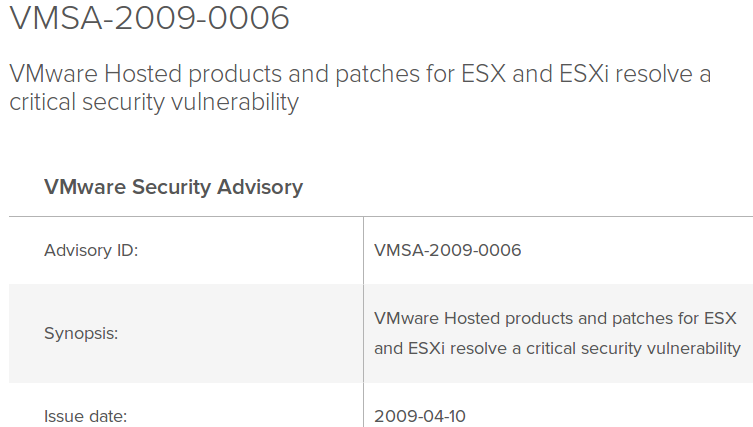
\includegraphics[width=0.7\textwidth]{vmware-vuln}


\includegraphics[width=\textwidth]{ars-venom}
\end{center}
\end{frame}

\begin{frame}{virtual machine escape}
\begin{itemize}
    \item bug in virtual machine monitor that lets virtual machines
          run code that's not isolated
\end{itemize}
\end{frame}

\subsection{VM detection: theory/practice}

\begin{frame}{VM detection}
\begin{tikzpicture}
\node[anchor=north west] (vmsurvey)  at (0,0){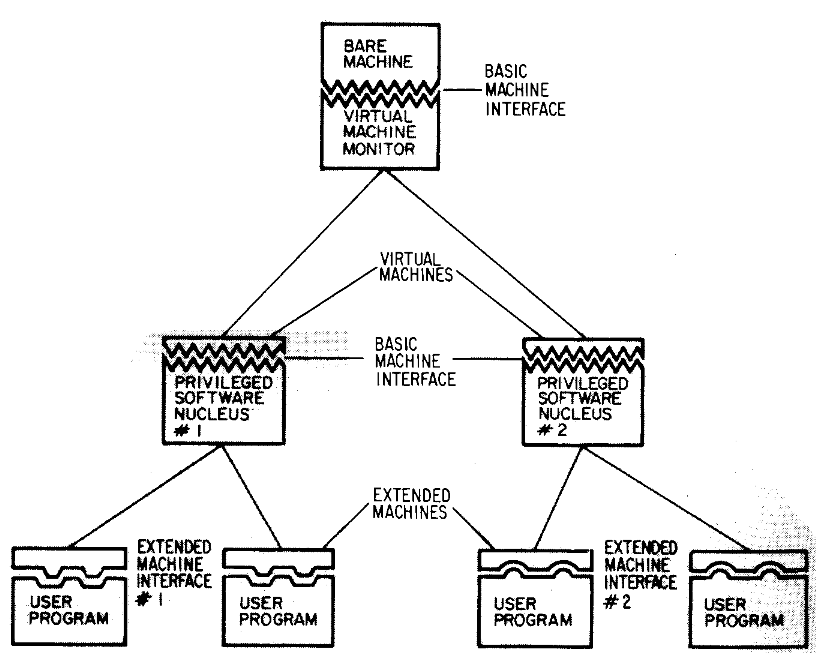
\includegraphics[height=.8\textheight]{VMSurvey-Fig2}};
%\draw[help lines] (0,0) grid (12, -8) ;
\draw[red, thick] (5.5, -.8) rectangle (6.5, -1.5);
\draw[red, thick] (4.3, -3.8) rectangle (5.3, -4.5);
\node[red, anchor=west] (sameQ) at (8, -2.5) {really the same?};
\draw[red, thick] (6.5, -1) -- (sameQ.west);
\draw[red, thick] (5.3, -4) -- (sameQ.west);
\end{tikzpicture}
\end{frame}

\begin{frame}{VM detection}
    \begin{itemize}
    \item no reason why detectable, but\ldots{}
    \item normal system VMs are not \myemph{not stealthy}
    \end{itemize}
\end{frame}


{ % all template changes are local to this group.
    \setbeamertemplate{navigation symbols}{}
    \begin{frame}[plain]
        \begin{tikzpicture}[remember picture,overlay]
            \node[at=(current page.center)] {
                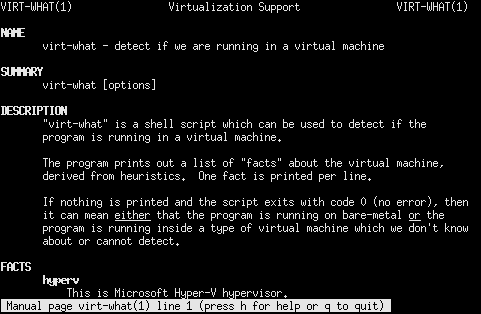
\includegraphics[width=\paperwidth]{virt-what-manpage}
            };
        \end{tikzpicture}
    \end{frame}
}

\begin{frame}[fragile,label=woTools]{without specialized tools}
\begin{Verbatim}[fontsize=\small,commandchars=Q\{\}]
ubuntu@ubuntu-xenial:~$ sudo dmidecode | head
# dmidecode 3.0
Getting SMBIOS data from sysfs.
SMBIOS 2.5 present.
10 structures occupying 450 bytes.
Table at 0x000E1000.

Handle 0x0000, DMI type 0, 20 bytes
BIOS Information
        Vendor: innotek Gmbcp 
        Version: Qtextbf{VirtualBox}
\end{Verbatim}
{\small DMI --- BIOS (system startup) table}
\end{frame}

\begin{frame}{VM detection: case study}
\begin{itemize}
    \item search for devices with ``VMWARE'' in their names
    \item search for VM-only device drivers
    \item check if processor is suspiciously slow
        \begin{itemize}
        \item ideally things that are easier in HW than SW
        \item e.g. speed of syscalls, address space changes
        \item unimplemented features?
        \item might need external source of time
        \end{itemize}
\end{itemize}
\imagecredit{Via \url{https://www.fireeye.com/blog/threat-research/2011/01/the-dead-giveaways-of-vm-aware-malware.html}} 
\end{frame}

\begin{frame}{VMs for anti-malware} 
\begin{itemize}
    \item does SW do something bad?
    \item run it in a VM/``sandbox''
    \item check if things change that shouldn't
    \item actual antivirus software technique
\end{itemize}
\end{frame}

\begin{frame}{VMs as antimalware limitations}
    \begin{itemize}
    \item completeness
        \begin{itemize}
        \item emulate entire filesystem?
        \item emulate all system calls?
        \item emulate network?
        \item provide real network?
        \end{itemize}
    \item user input, etc.
        \begin{itemize}
        \item can't easily automate keypresses, etc.
        \end{itemize}
    \item speed
        \begin{itemize}
        \item how long until you say ``it's safe''
        \end{itemize}
    \end{itemize}
\end{frame}

\begin{frame}{lightweight sandboxing}
\begin{itemize}
    \item (system) VMs are resource-intensive
    \item \myemph{two OSes} --- lots of extra memory
    \item worse performance
        \begin{itemize}
        \item more code needed for I/O
        \end{itemize}
    \vspace{1cm}
    \item more efficient alternative: operating system isolation
        \begin{itemize}
        \item e.g. on lab machines, users can't interfere with each other
        \item e.g. browsers do this for web page code
    \end{itemize}
\end{itemize}
\end{frame}


\begin{frame}{OS interface size}
% FIXME: syscall counts
% FIXME: complicated states?
% FIXME: # of drivers
    \begin{itemize}
    \item OS interfaces are \myemph{complicated}
    \item Linux:
        \begin{itemize}
        \item 100s of system calls
        \item \ldots{} including some to talk to hundreds of device drivers
        \end{itemize}
    \item hard to tell which program needs
    \item hard to tell which are safe
    \end{itemize}
\end{frame}

\begin{frame}{OS sandboxing support}
    \begin{itemize}
    \item OS-level isolation of filesystem, memory, CPU
    \item extra code for each kind of resource/system call
    \item lots of obscure system resources to exhaust, etc.:
        \begin{itemize}
        \item list of pending signals
        \item network buffers
        \item buffers for interprocess pipes
        \item process control data structures in the OS
        \item etc.
        \end{itemize}
    \item need to limit each of them
    \end{itemize}
\end{frame}

\begin{frame}{sandboxing on Linux (1)}
    \begin{itemize}
    \item one mechanism: secccomp
    \item \myemph{system call filter}
    \item example: video decoder:
        \begin{itemize}
        \item reads encoded video
        \item writes decoded images
        \end{itemize}
    \item only needs read/write --- easy to sandbox
    \end{itemize}
\end{frame}

\begin{frame}{sandboxing on Linux (2)}
    \begin{itemize}
    \item another mechanism: cgroups
    \item set limits for CPU, memory, networks, process IDs, etc.
    \item \myemph{extra kernel code} for each kind of resource
    \item only expose subset of filesystem ({\tt chroot})
        \begin{itemize}
        \item {\tt /} (root directory) changedA
        \end{itemize}
    \item \textbf{much} more complex to configure securely than VM
    \item not used by major rental computing providers
    \end{itemize}
\end{frame}

\begin{frame}{the real sandboxing problem}
    \begin{itemize}
    \item policy
    \end{itemize}
\end{frame}


\begin{frame}{VMs in this course}
    \begin{itemize}
    \item consistent environment!
    \item our attacks may depend on \myemph{exact memory addresses}
    \item our attacks may depend on \myemph{exact versions of system libraries}
    \end{itemize}
\end{frame}

\begin{frame}{do real attackers do that?}
    \begin{itemize}
    \item if exploits are so sensitive\ldots
    \vspace{.5cm}
    \item fragile, not always broken
    \item exploits can be made less fragile
    \item Slapper worm: exploit variants for 23 architectures
    \end{itemize}
\end{frame}

\begin{frame}{exploits: avoiding fragility}
    \begin{itemize}
    \item some exploits cause a jump to attacker-controlled code
    \item fragile because need to encode \myemph{exact address}
    \item partial fix: choose exploit code to give leeway
    \end{itemize}
\end{frame}

\begin{frame}[fragile,label=nopSled]{nop sled}
\begin{lstlisting}[style=small,language=myasm]
nop  /* <- jumping to here */
nop
nop
nop
nop
nop  /* <- same as jumping to here */
nop
nop
...
/* exploit code here */
\end{lstlisting}
\end{frame}

% FIXME: insert some assembly slides here

\begin{frame}{next topic: x86-64 assembly}
    \begin{itemize}
    \item you've seen this before
    \item in theory
    \end{itemize}
\end{frame}

\begin{frame}{x86-64 assembly}
\begin{itemize}
\item history: AMD constructed 64-bit extension to x86 first
    \begin{itemize}
    \item marketing term: AMD64
    \end{itemize}
\item Intel first tried a new ISA (Itanium), which failed
\item Then Intel copied AMD64
    \begin{itemize}
    \item marketing term: EM64T (Extended Memory 64 Technology)
    \item later marketing term: Intel 64
    \end{itemize}
\item both Intel and AMD have manuals --- definitive reference
\end{itemize}
\end{frame}

\begin{frame}
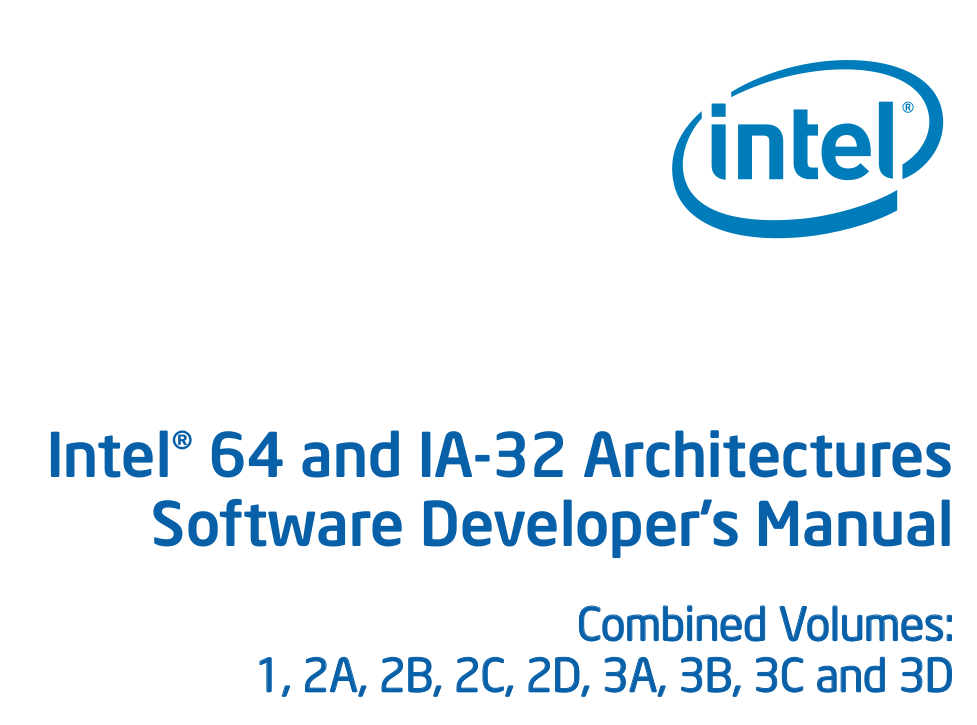
\includegraphics[height=0.9\textheight]{manual-screenshot}
\end{frame}

\begin{frame}{x86-64 manuals}
\begin{itemize}
\item Intel manuals:
    \begin{itemize}
    \item \small \url{https://software.intel.com/en-us/articles/intel-sdm}
    \item 24 MB, 4684 pages
    \item Volume 2: instruction set reference (2190 pages)
    \end{itemize}
\item AMD manuals:
    \begin{itemize}
    \item \small \url{https://support.amd.com/en-us/search/tech-docs}
    \item ``AMD64 Architecture Programmer's Manual''
    \end{itemize}
\end{itemize}
\end{frame}

\begin{frame}{recall: x86-64 general purpose registers}
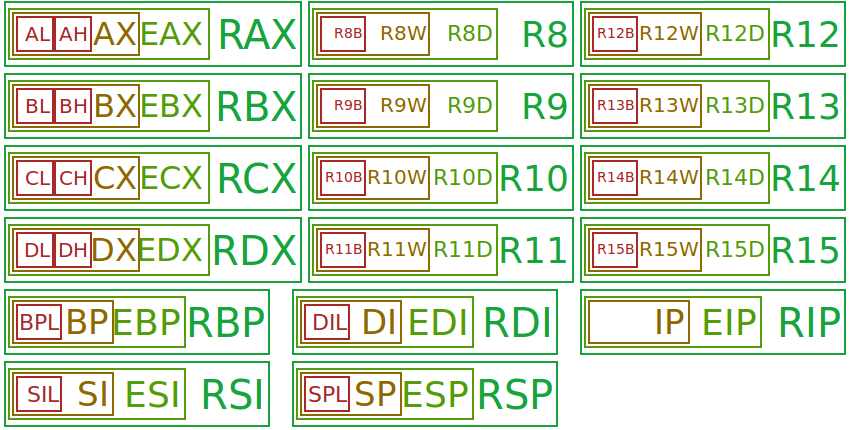
\includegraphics[width=\textwidth]{x86-gprs}
\imagecredit{Immae via Wikipedia}
\end{frame}

\begin{frame}[fragile,label=overlap]{overlapping registers (1)}
\begin{itemize}
\item setting 32-bit registers sets \myemph{whole} 64-bit register
\item extra bits are always zeroes
\end{itemize}
\begin{lstlisting}[style=small]
movq $0x123456789abcdef, %rax
xor %eax, %eax
// %rax is 0, not 0x1234567800000000
movl $-1, %ebx
// %rbx is 0xFFFFFFFF, not -1 (0xFFFFFFFFFFFFFFFF)
\end{lstlisting}
\end{frame}

\begin{frame}[fragile,label=overlap2]{overlapping registers (2)}
\begin{itemize}
\item setting \myemph{8/16-bit registers} doesn't change rest of 64-bit register:
\end{itemize}
\begin{lstlisting}[style=small]
movq $0x12345789abcdef, %rax
movw $0xaaaa, %ax
// %rax is 0x123456789abaaaa
\end{lstlisting}
\end{frame}

% FIXME: manual screenshots

\section{AT\&T versus Intel}

\begin{frame}{AT\&T versus Intel syntax}
    \begin{itemize}
    \item AT\&T syntax: \\ {\tt movq \$42, 100(\%rbx,\%rcx,4)}
    \item Intel syntax: \\ {\tt mov QWORD PTR [rbx+rcx*4+100], 42}
    \item effect (pseudo-C): \\ {\tt memory[rbx + rcx * 4 + 100] <- 42}
    \end{itemize}
\end{frame}

\begin{frame}[fragile,label=att1]{AT\&T syntax (1)}
\begin{lstlisting}
movq $42, 100(%rbx,%rcx,4)
\end{lstlisting}
    \begin{itemize}
    \item destination \myemph{last}
    \item constants start with {\tt \$}
    \item registers start with {\tt \%}
    \end{itemize}
\end{frame}

\begin{frame}[fragile,label=att2]{AT\&T syntax (2)}
\begin{lstlisting}
movq $42, 100(%rbx,%rcx,4)
\end{lstlisting}
    \begin{itemize}
    \item operand length: {\tt q}
        \begin{itemize}
        \item {\tt l} = 4; {\tt w} = 2; {\tt b} = 1
        \item 
        \end{itemize}
    \item {\tt 100(\%rbx,\%rcx,4)}: \\ {\tt memory[100 + rbx + rcx * 4]}
    \item {\tt sub \%rax, \%rbx}: {\tt rbx $\leftarrow$ rbx - rax}
    \end{itemize}
\end{frame}

\begin{frame}{Intel syntax}
    \begin{itemize}
    \item destination \myemph{first}
    \item {\tt [...]} indicates location in memory
    \item {\tt QWORD PTR [...]} for 8 bytes in memory
        \begin{itemize}
        \item DWORD for 4
        \item WORD for 2
        \item BYTE for 1
        \end{itemize}
    \end{itemize}
\end{frame}

% FIXME: move this?
\begin{frame}[fragile,label=LEA]{On LEA}
    \begin{itemize}
    \item LEA = Load Effective Address
    \item uses the syntax of a memory access, but\ldots{}
    \item just computes the address and uses it:
    \item ~ \lstinline|leaq 4(%rax), %rax| has same result as \lstinline|addq $4, %rax|
        \begin{itemize}
        \item almost --- doesn't set condition codes
        \end{itemize}
    \item ~ \lstinline|leaq (%rax,%rax,4), %rax| multiplies {\tt \%rax} by 5
        \begin{itemize}
        \item {\tt address-of(memory[rax + rax * 4])}
        \end{itemize}
    \end{itemize}
\end{frame}

\begin{frame}[fragile,label=question]{question}
\lstset{style=small}
\begin{lstlisting}
.data
string:
    .asciz "abcdefgh"
.text
    movq $string, %rax
    movq string, %rdx
    movb (%rax), %bl
    leal 1(%rbx), %ebx
    movb %bl, (%rax)
    movq %rdx, 4(%rax)
\end{lstlisting}
{\small What is the final value of string?}
\begin{itemize}
\item a. "abcdabcd"
\item b. "bbcdefgh"
\item c. "bbcdabcd"
\item d. "abcdefgh"
\item e. something else / not enough info
\end{itemize}
\end{frame}

